\begin{ledgroupsized}[r]{120mm}
\footnotesize
\pstart
\noindent\textbf{\"{U}berlieferung:}
\pend
\end{ledgroupsized}
\begin{ledgroupsized}[r]{114mm}
\footnotesize
\pstart \parindent -6mm
\makebox[6mm][l]{\textit{L?}}%
LH XXXV 12, 2 Bl. 86. Ein Blatt 4\textsuperscript{o}; Teil eines Wasserzeichens. Zwei Seiten; Zeichnung auf Bl. 86~r\textsuperscript{o}; Bl. 86~v\textsuperscript{o} leer.
\\ Cc 2, Nr. 1559
\pend
\end{ledgroupsized}
\vspace{5mm}
\begin{ledgroup}
\footnotesize
\pstart
\noindent\footnotesize{\textbf{Datierungsgr\"{u}nde}: Das Wasserzeichen ist für den in der Datierung angegebenen Zeitraum belegt.}
\pend
\end{ledgroup}

\vspace{5mm}
\pstart\noindent
[86~r\textsuperscript{o}] 
\vspace{0.5em}
\pend
\centerline{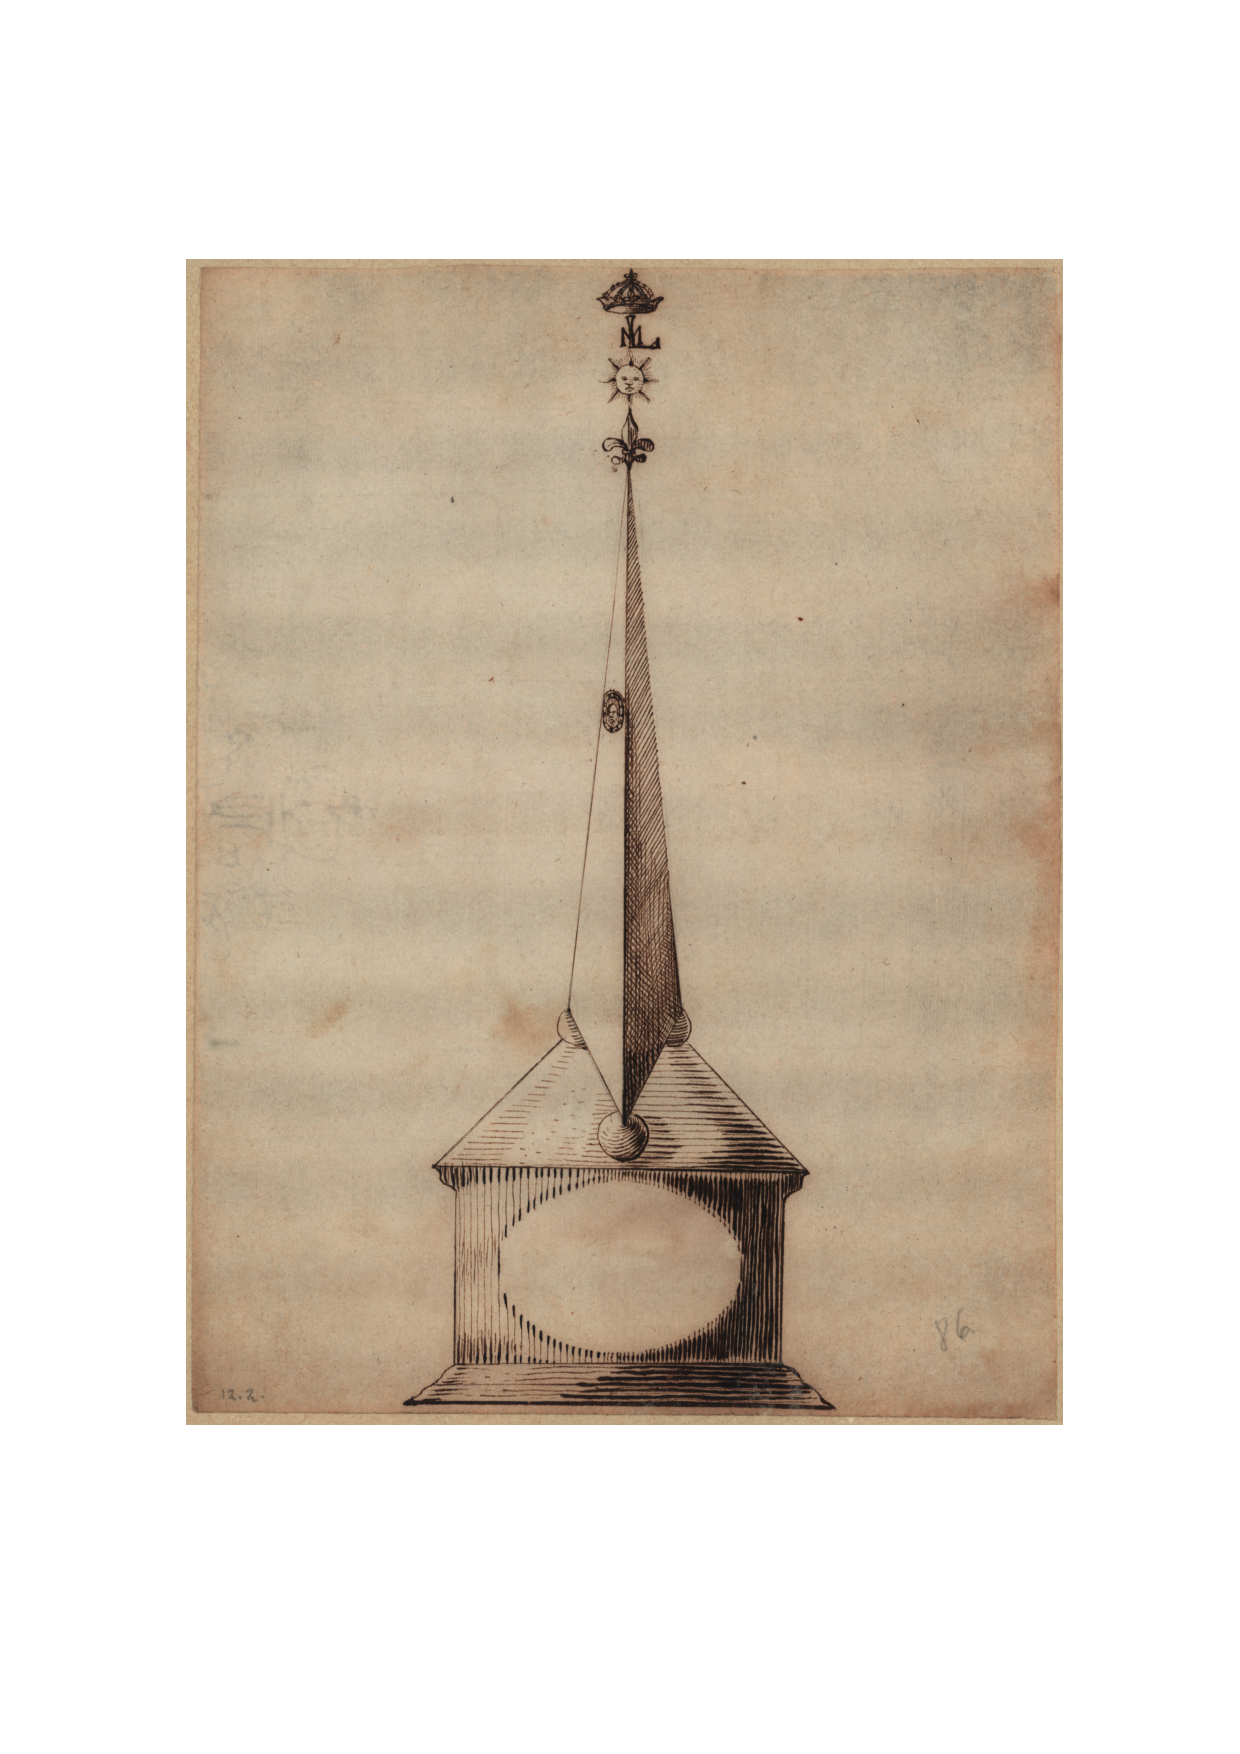
\includegraphics[width=0.5\textwidth]{gesamttex/edit_VIII,3/images/LH_35_12_02_086_d.pdf}}
%\vspace*{-0.3em}
\centerline{\lbrack\textit{Fig.~1}\rbrack}
%\vspace{0.5em}
%LH35_12_00_02_00_00_0056_1_1
\count\Afootins=1200%
\count\Bfootins=1200%
\count\Cfootins=1200